\documentclass[12pt,a4paper]{article}
\usepackage[utf8x]{inputenc}
\usepackage{ucs}
\usepackage{amsmath}
\usepackage{amsfonts}
\usepackage{amssymb}
\usepackage{graphicx}
\usepackage{grffile}
\usepackage{float}
\usepackage{multicol}
\usepackage[portuguese]{babel}
\title{Dinamica}
\author{André Garnier Coutinho}
\setlength{\textwidth}{17cm}
\setlength{\textheight}{24cm}
\addtolength{\topmargin}{-2cm}
\addtolength{\oddsidemargin}{-2cm}
\begin{document}
\begin{center}
\textbf{Escola Politécnica da USP\\
IC2014 - Grupo de pesquisa em Robótica e suas aplicações\\}
\end{center}

\begin{center}
\textbf{Dinâmica}
\end{center}

\noindent{\bf Algumas definições importantes: \\}

Seja $\mho$ um sistema mecânico de $n$ graus de liberdade. Para encontrar as equações diferenciais de movimento do sistema, é conveniente fazer as seguintes definições:

\begin{itemize}
\item[•]$q^{\#}$: vetor de $n$ coordenadas generalizadas independentes
\item[•]$q^o$: vetor de $m_q$ coordenadas generalizadas redundandes
\item[•]$q$: vetor contendo todas as coordenadas generalizadas. Usualmente $q = \begin{bmatrix} q^{\#} \\q^o \end{bmatrix} $
\item[•]$\phi(q)$: vetor de tamanho $m_q$ dos vínculos de posição, de modo que conhecendo $q^{\#}$ seja possível determinar $q^o$ resolvendo $\phi(q) = 0$
\item[•]$p^{\#}$: vetor de $n$ velocidades generalizadas independentes
\item[•]$p^o$: vetor de $m_p$ velocidades generalizadas redundandes
\item[•]$p$: vetor contendo todas as velocidades generalizadas. Usualmente $p = \begin{bmatrix} p^{\#} \\p^o \end{bmatrix} $
\item[•]$\Lambda(q,p)$: vetor de tamanho $m_q$ dos vínculos de velocidades, de modo que conhecendo $q$ e $p^{\#}$ seja possível determinar $p^o$ resolvendo $\Lambda(q,p) = 0$
\item[•]$f_q$ vetor de $n+m_q$ esforços ativos dos atuadores na direção $q$ (${f_q}_i$ está na direção de $q_i, i = 1,2,...,n+m_q$)
\item[•]$f_p$ vetor de $n+m_p$ esforços ativos dos atuadores na direção $p$ (${f_p}_i$ está na direção de $p_i, i = 1,2,...,n+m_p$)
\item[•]$F_q$ vetor de $n+m_q$ esforços ativos dos atuadores na direção $q^{\#}$ (${f_q}_i$ está na direção de $q_i, i = 1,2,...,n$)
\item[•]$F_p$ vetor de $n+m_p$ esforços ativos dos atuadores na direção $p^{\#}$ (${f_p}_i$ está na direção de $p_i, i = 1,2,...,n$)
\end{itemize}

Na dinâmica de sistemas mecânicos multi-corpos, é muito vantajosa a utilização de coordenadas/velocidades generalizadas redundantes, pois a utilização destas diminui a complexidade da utilização dos métodos de dedução das equações de movimento (como Lagrange, Kane e Gibbs-Appell) e em contrapartida aumenta a complexidade da cinemática (pois torna necessário definir $\phi(q)$ e $\Lambda(q,p)$). \\

Nos métodos citados, é necessário o cálculo das velocidades absolutas dos centros de massa $\vec{v}_{G_i}$ e das velocidades angulares absolutas $\vec{\omega}_i$ de todos os corpos rígidos do sistema, em função de $p$ e $q$. Sendo assim, é conveniente definir o vetor de velocidades generalizadas $p$ como sendo todas as componentes dos $\vec{v}_{G_i}$ e dos $\vec{\omega}_i$, em alguma ordem conveniente. Fazendo isso, tornamos a apliação dos métodos extremamente simples, deixando praticamente toda a complexidade do problema no cálculo de $\phi(q)$ e $\Lambda(q,p)$. \\

Aqui seguem sugestões de escolhas de coordenadas $q$ e $p$:
\begin{itemize}
\item[•] Para mecanismo seriais:
	\begin{itemize}
	\item[-] Escolher $q^{\#}$ como sendo as coordenadas relativas das juntas atuadas (ângulos de giro para juntas ativas de rotação e deslocamentos lineares para juntas ativas prismáticas) e $q^o$ como sendo as coordenadas dos centros de massa das barras do mecanismos em relação a um referencial inercial.
	
	\item[-] Escolher $p$ como sendo todas as componentes de $[\vec{v}_{G_i}]_{B_i}$ e dos $[\vec{\omega}_i]_{B_i}$, $i = 1, 2, ..., n$, sendo $B_i$ um sistema de coordenadas cartesianos preso na i-ésima barra, cujos eixos são paralelos às direções principais da i-ésima barra.
As coordenadas $p^{\#}$ serão as componentes de $p$ análogas a $\dot{q}^{\#}$, com a diferença que serão velocidades absolutas.

	\end{itemize}


\noindent{\bf Exemplo 1 \\}

\begin{figure}[h!]
	\centering
	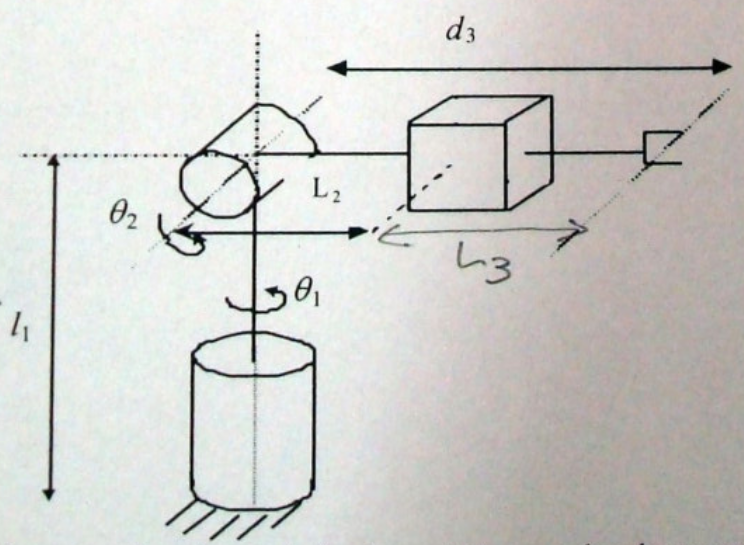
\includegraphics[scale=0.4]{RRP.png}  
	\caption{Robô \underline{R}\underline{R}\underline{P}}
	\label{fig:figura1}
\end{figure}

\begin{itemize}

\item[-] Primeiro definimos $n + m_q$ coordenadas  $q$. Estas podem ser subdivididas em $n$ coordenadas independentes $q^{\#}$ e $m_q$ coordenadas redudantes $q^o$.

$$ q = \begin{bmatrix}
q^{\#} \\
q^o
\end{bmatrix} $$

No caso do mecanismo $\underline{R}\underline{R}\underline{P}$, temos:




$$ q^{\#} = \begin{bmatrix}
\theta_1 & \theta_2 & d_3
\end{bmatrix}^T $$
$$ q^o = \begin{bmatrix}
x_1 & y_1 & z_1 & x_2 & y_2 & z_2 & x_3 & y_3 & z_3 
\end{bmatrix}^T $$

Com $n = 3$ e $m_q = 9$. Neste caso, as componentes de $q^o$ são as coordenadas dos centros de massa das barras, escritas no referencial canônico. \\

\item[-] Depois definimos $n + m_p$ coordenadas  $p$. Estas podem ser subdivididas em $n$ coordenadas independentes $p^{\#}$ e $m_p$ coordenadas redudantes $p^o$. As coordenadas $p^{\#}$ podem ser subdividas em $n_1$ velocidades angulares $\omega^{\#}$ e $n_2$ velocidades lineares $v^{\#}$. As coordenadas $p^o$ podem ser subdividas em $m_{p1}$ velocidades angulares $\omega^o$ e $m_{p2}$ velocidades lineares $v^o$.

\begin{multicols}{3}
$ p = \begin{bmatrix}
p^{\#} \\
p^o
\end{bmatrix} $

$ p^{\#} = \begin{bmatrix}
\omega^{\#} \\
v^{\#}
\end{bmatrix} $



$ p^o = \begin{bmatrix}
\omega^o \\
v^o
\end{bmatrix} $

\end{multicols}

No caso do mecanismo $\underline{R}\underline{R}\underline{P}$, temos:


$$ \omega^{\#} = \begin{bmatrix}
\omega_{z1} \\
\omega_{x2}
\end{bmatrix} $$
$$ v^{\#} = \begin{bmatrix}
v_{y3}
\end{bmatrix} $$
$$ \omega^o = \begin{bmatrix}
\omega_{x1} & \omega_{y1} & \omega_{y2} & \omega_{z2} & \omega_{x3} & \omega_{y3} & \omega_{z3}
\end{bmatrix}^T $$
$$ v^o = \begin{bmatrix}
v_{x1} & v_{y1} & v_{z1} & v_{x2} & v_{y2} & v_{z2} & v_{x3} & v_{z3}
\end{bmatrix}^T $$

Com $m_{p1} = 7$, $m_{p2} = 8$ e $m_p = m_{p1} + m_{p2} = 15$, sendo $v^{\#}$ e $v^o$ as componentes das velocidades absolutas dos centros de massa das barras, escritas nas bases presas às barras, e $\omega^{\#}$ e $\omega^o$ as componentes das velocidades angulares absolutas, escritas nas bases presas às barras.

\end{itemize}


\item[•] Para mecanismos paralelos:

\begin{itemize}
	\item[-] Escolher $q$ como sendo as coordenadas relativas das juntas atuadas, as coordenadas dos centros de massa das barras do mecanismos em relação a um referencial inercial, os deslocamentos angulares ou lineares (relativos ou absolutos) das juntas passivas não conectadas diretamente à plataforma, e as coordenadas do centro de massa e orientação da plataforma em relação a um referencial inercial. Se fizer sentido e for conveniente, podem ser escolhidas $n$ coordenadas dentro destas para formarem as coordenadas $q^{\#}$.
\end{itemize}

	\item[-] Escolher $p$ como sendo todas as componentes das velocidades absolutas dos centros de massa e das velocidades angulares de todos os corpos rígidos do sistema. As coordenadas $p^{\#}$ serão as componentes não nulas da velocidade absoluta do centros de massa e das velocidades angulares absolutas da plataforma. 



\noindent{\bf Exemplo 2 \\}

Exemplo de mecanismo paralelo

\begin{itemize}
\item[-]
\item[-]
\end{itemize}

\end{itemize}

Quanto ao cálculo do vetor $\phi(q)$ dos vínculos de posição, realizamos o seguinte procedimento:
\begin{itemize}
\item[•] Para mecanismos seriais:
	\begin{itemize}
	\item[-] Basta utilizar matrizes de transformação homogênea para relacionar as coordenadas dos centros de massa das barras (em relação a 	uma base 	fixa) com os deslocamentos angulares ou lineares das juntas ativas.	
	\end{itemize}


\noindent{\bf Exemplo 3 \\}

\begin{itemize}

\item[-] Realizamos a cinemática de posição para os centros de massa das barras, de modo a relacionar as coordenadas $q^o$ com as coordenadas $q^{\#}$. Para isso, utilizamos matrizes de transformação homogênea.



$$ [H]_{B_1/can} =
\begin{bmatrix}
 Rot(\theta_1, z_0) & [\overrightarrow{O_0 O_1}]_{can} \\
 0_{3x1} & 1 \\
\end{bmatrix}
=
\begin{bmatrix}
 c_1 & -s_1 & 0 & 0 \\
 s_1 & c_1 & 0 & 0 \\
 0 & 0 & 1 & h \\
 0 & 0 & 0 & 1 \\
\end{bmatrix} ;
\begin{bmatrix}
[\overrightarrow{O_1 G_1}]_{B_1} \\
1
\end{bmatrix}
=
\begin{bmatrix}
0 \\
0 \\
l_{1g} \\
1 \\
\end{bmatrix}
$$

$$ [H]_{B_2/B_1} =
\begin{bmatrix}
 Rot(\theta_2, x_1) & [\overrightarrow{O_1 O_2}]_{B_1} \\
 0_{3x1} & 1 \\
\end{bmatrix}
=
\begin{bmatrix}
 1 & 0 & 0 & 0 \\
 0 & c_2 & -s_2 & 0 \\
 0 & s_2 & c_2 & l_1 \\
 0 & 0 & 0 & 1 \\
\end{bmatrix} ;
\begin{bmatrix}
[\overrightarrow{O_2 G_2}]_{B_2} \\
1
\end{bmatrix}
=
\begin{bmatrix}
0 \\
l_{2g} \\
0 \\
1 \\
\end{bmatrix}
$$

$$ [H]_{B_3/B_2} =
\begin{bmatrix}
 I_{3x3} & [\overrightarrow{O_2 O_3}]_{B_2} \\
 0_{3x1} & 1 \\
\end{bmatrix}
=
\begin{bmatrix}
 1 & 0 & 0 & 0 \\
 0 & 1 & 0 & l_2 \\
 0 & 0 & 1 & 0 \\
 0 & 0 & 0 & 1 \\
\end{bmatrix} ;
\begin{bmatrix}
[\overrightarrow{O_3 G_3}]_{B_3} \\
1
\end{bmatrix}
=
\begin{bmatrix}
0 \\
d_3-l_3+l_{3g} \\
0 \\
1 \\
\end{bmatrix}
$$ \\

$$
[H]_{B_2/can} = [H]_{B_1/can} [H]_{B_2/B_1} =
 \begin{bmatrix}
 c_1 & -c_2 s_1 & s_1 s_2 & 0 \\
 s_1 & c_1 c_2 & -c_1 s_2 & 0 \\
 0 & s_2 & c_2 & h+l_1 \\
 0 & 0 & 0 & 1 \\
\end{bmatrix}
$$

$$
[H]_{B_3/can} = [H]_{B_2/can} [H]_{B_3/B_2} =
\begin{bmatrix}
 c_1 & -c_2 s_1 & s_1 s_2 & -c_2 s_1 l_2 \\
 s_1 & c_1 c_2 & -c_1 s_2 & c_1 c_2 l_2 \\
 0 & s_2 & c_2 & h+l_1+s_2 l_2 \\
 0 & 0 & 0 & 1 \\
\end{bmatrix}
$$





$$ \therefore \begin{bmatrix}
x_1 \\
y_1 \\
z_1 \\
1 \\
\end{bmatrix}
=
[H]_{B_1/can}
\begin{bmatrix}
[\overrightarrow{O_1 G_1}]_{B_1} \\
1
\end{bmatrix}
=
\begin{bmatrix}
 0 \\
 0 \\
 h+l_{\text{1g}} \\
 1 \\
\end{bmatrix}
$$

$$ \begin{bmatrix}
x_2 \\
y_2 \\
z_2 \\
1 \\
\end{bmatrix}
=
[H]_{B_2/can}
\begin{bmatrix}
[\overrightarrow{O_2 G_2}]_{B_2} \\
1
\end{bmatrix}
=
\begin{bmatrix}
 -c_2 s_1 l_{2g} \\
 c_1 c_2 l_{2g} \\
 h+l_1+s_2 l_{2g} \\
 1 \\
\end{bmatrix}
$$

$$ \begin{bmatrix}
x_3 \\
y_3 \\
z_3 \\
1 \\
\end{bmatrix}
=
[H]_{B_3/can}
\begin{bmatrix}
[\overrightarrow{O_3 G_3}]_{B_3} \\
1
\end{bmatrix}
=
\begin{bmatrix}
 -c_2 s_1 (l_2-l_3+l_{3g}+d_3) \\
 c_1 c_2 (l_2-l_3+l_{3g}+d_3) \\
 h+l_1+s_2 (l_2-l_3+l_{3g}+d_3) \\
 1 \\
\end{bmatrix}
$$

Repare que a partir das matrizes de transformação homogênea encontradas, encontramos também as seguintes matrizes de mudança de base:

$$ R_1 = [I]_{B_1/can} =  \begin{bmatrix}
 c_1 & -s_1 & 0 \\
 s_1 & c_1 & 0 \\
 0 & 0 & 1 \\
\end{bmatrix} $$

$$ R_2 = [I]_{B_2/can} =  \begin{bmatrix}
 c_1 & -c_2 s_1 & s_1 s_2 \\
 s_1 & c_1 c_2 & -c_1 s_2 \\
 0 & s_2 & c_2 \\
\end{bmatrix}
= R_3 = [I]_{B_3/can} $$

Com a cinemática de posição, conseguimos obter $m_q = 9$ equações vínculares de posição. Sendo assim, o vetor dos vínculos de posição é dado por:

$$
\phi(q)
=
\begin{bmatrix}
x_1  \\
y_1 \\
z_1 - h - l_{1g} \\
x_2 + c_2 s_1 l_{2g} \\
y_2 - c_1 c_2 l_{2g}\\
z_2 -h - l_1 - s_2 l_{2g}\\
x_3 + c_2 s_1 (l_2-l_3+l_{3g}+d_3) \\
y_3 - c_1 c_2 (l_2-l_3+l_{3g}+d_3) \\
z_3 - h - l_1 - s_2 (l_2-l_3+l_{3g}+d_3)\\
\end{bmatrix}
$$

\end{itemize}

\item[•] Para mecanismos paralelos:
	\begin{itemize}
	
	\item[-] Utilizar matrizes de transformação homogênea para relacionar as coordenadas dos centros de massa das barras (em relação a uma 		base fixa) com os deslocamentos angulares e/ou lineares das juntas ativas e passivas
	\item[-] Utilizar equações de loop fechado e/ou equações que relacionem diretamente as coordenadas atuadas com as coordenadas da 				plataforma para completar as $m_q$ equações viculares.

	\end{itemize}
\noindent{\bf Exemplo 4 \\}

Exemplo de mecanismo paralelo

\begin{itemize}
\item[-]
\item[-]
\end{itemize}

Quanto ao cálculo do vetor $\Lambda(q,p)$ dos vínculos de velocidades, realizamos o seguinte procedimento:
\begin{itemize}

\item[•] Para mecanismos seriais:

	\begin{itemize}
	\item[-] Utilizar as matrizes de rotação para o cálculo das velocidades angulares nas bases presas às barras
	\item[-] Derivar as coordenadas dos centros de massa para encontrar os vetores velocidade absoluta na base canônica
	\item[-] Utilizar as matrizes de rotação para mudar os vetores velocidade absoluta para as bases presas às barras
	\item[-] Montar os vetores $p^{\#}$ em função de $q^{\#}$ e $\dot{q}^{\#}$ ($P^{\#} (q^{\#}, \dot{q}^{\#} )$) e $p^o$ em função de 			$q^{\#}$ e $\dot{q}^{\#}$ ($P^o (q^{\#}, \dot{q}^{\#} )$)
	\item[-]  Utilizar a linearidade de $P^{\#} (q^{\#}, \dot{q}^{\#} )$ e $P^o (q^{\#}, \dot{q}^{\#} )$ em relação a $\dot{q}^{\#}$ para 			encontrar os vínculos de velocidades
	\end{itemize}

\noindent{\bf Exemplo 5 \\}


\begin{itemize}
\item[-] Utilizamos as matrizes de rotação para calcular as velocidades angulares em função de $q^{\#}$ e $\dot{q}^{\#}$:

$$ [S(\vec{\omega}_1)]_{B_1} = R_1^T \dot{R}_1 =
\begin{bmatrix}
0 & -\dot{\theta}_1 & 0 \\
\dot{\theta}_1 & 0 & 0 \\
0 & 0 & 0 \\
\end{bmatrix}
\Rightarrow
[\vec{\omega}_1]_{B_1} =
\begin{bmatrix}
0 \\
0 \\
\dot{\theta}_1
\end{bmatrix}
$$

$$ [S(\vec{\omega}_2)]_{B_2} = R_2^T \dot{R}_2 =
\begin{bmatrix}
0 & -c_2 \dot{\theta}_1 & s_2 \dot{\theta}_1 \\
c_2 \dot{\theta}_1 & 0 & -\dot{\theta}_2 \\
-s_2 \dot{\theta}_1 & \dot{\theta}_2 & 0 \\
\end{bmatrix}
\Rightarrow
[\vec{\omega}_1]_{B_2} =
\begin{bmatrix}
\dot{\theta}_2 \\
s_2 \dot{\theta}_1 \\
c_2 \dot{\theta}_1
\end{bmatrix}
$$

$$ [S(\vec{\omega}_3)]_{B_3} = R_3^T \dot{R}_3 =
\begin{bmatrix}
0 & -c_2 \dot{\theta}_1 & s_2 \dot{\theta}_1 \\
c_2 \dot{\theta}_1 & 0 & -\dot{\theta}_2 \\
-s_2 \dot{\theta}_1 & \dot{\theta}_2 & 0 \\
\end{bmatrix}
\Rightarrow
[\vec{\omega}_3]_{B_3} =
\begin{bmatrix}
\dot{\theta}_2 \\
s_2 \dot{\theta}_1 \\
c_2 \dot{\theta}_1
\end{bmatrix}
$$

\item[-] Derivamos as equações de posição para encontrar as velocidades dos centros de massa:

$$
[\vec{v}_1]_{can} =
\begin{bmatrix}
\dot{x}_1 \\
\dot{y}_1 \\
\dot{z}_1
\end{bmatrix}
=
\begin{bmatrix}
0 \\
0 \\
0
\end{bmatrix}
$$

$$
[\vec{v}_2]_{can} =
\begin{bmatrix}
\dot{x}_2 \\
\dot{y}_2 \\
\dot{z}_2
\end{bmatrix}
=
\begin{bmatrix}
l_{2g} ( \dot{\theta}_2 s_1 s_2 - \dot{\theta}_1 c_1 c_2 ) \\
-l_{2g} ( \dot{\theta}_1 s_1 c_2 - \dot{\theta}_2 c_1 s_2 ) \\
l_{2g} \dot{\theta}_2 c_2 
\end{bmatrix}
$$

$$
[\vec{v}_3]_{can} =
\begin{bmatrix}
\dot{x}_3 \\
\dot{y}_3 \\
\dot{z}_3
\end{bmatrix}
=
\begin{bmatrix}
-\dot{d}_3 s_1 c_2 - (d_3 + l_{3g} + l_2 - l_3)(\dot{\theta}_1 c_1 c_2 - \dot{\theta}_2 s_1 s_2) \\
\dot{d}_3 c_1 c_2 - (d_3 + l_{3g} + l_2 - l_3)(\dot{\theta}_1 s_1 c_2 - \dot{\theta}_2 c_1 s_2) \\
\dot{\theta}_2 c_2 (d_3 + l_{3g} + l_2 - l_3) + \dot{d}_3 s_2
\end{bmatrix}
$$

\item[-] Passamos as velocidades dos centros de massa para as bases pesas nas barras:

$$
[\vec{v}_1]_{B_1} = [I]_{can/B_1} [\vec{v}_1]_{can} = R_1^T [\vec{v}_1]_{can} = 
\begin{bmatrix}
v_{x1} \\
v_{y1} \\
v_{z1} 
\end{bmatrix}
= \vec{0}
$$

$$
[\vec{v}_2]_{B_2} = [I]_{can/B_2} [\vec{v}_2]_{can} = R_2^T [\vec{v}_2]_{can} =
\begin{bmatrix}
v_{x2} \\
v_{y2} \\
v_{z2} 
\end{bmatrix}
=
\begin{bmatrix}
c_2 l_{2g} \dot{\theta}_1  \\
0 \\
l_{2g} \dot{\theta}_2
\end{bmatrix}
$$

$$
[\vec{v}_3]_{B_3} = [I]_{can/B_3} [\vec{v}_3]_{can} = R_3^T [\vec{v}_3]_{can} =
\begin{bmatrix}
v_{x3} \\
v_{y3} \\
v_{z3} 
\end{bmatrix}
=
\begin{bmatrix}
-c_2 (l_2 - l_3 + l_{3g} + d_3) \dot{\theta}_1 \\
\dot{d}_3 \\
(l_2 - l_3 + l_{3g} + d_3) \dot{\theta}_2
\end{bmatrix}
$$

\item[-] Montamos os vetores $p^{\#}$ e $p^o$ em função de $q^{\#}$ e $\dot{q}^{\#}$:

$$
p^{\#} = 
\begin{bmatrix}
\omega_{z1} \\
\omega_{x2} \\
v_{y3} \\
\end{bmatrix}
= P^{\#} (q^{\#}, \dot{q}^{\#} ) =
\begin{bmatrix}
\dot{\theta}_1 \\
\dot{\theta}_2 \\
\dot{d}_3
\end{bmatrix}
$$

$$
p^o = 
\begin{bmatrix}
\omega_{x1} \\
\omega_{y1} \\
\omega_{y2} \\
\omega_{z2} \\
\omega_{x3} \\
\omega_{y3} \\
\omega_{z3} \\
v_{x1} \\
v_{y1} \\
v_{z1} \\
v_{x2} \\
v_{y2} \\
v_{z2} \\
v_{x3} \\
v_{z3} 
\end{bmatrix}
= P^o (q^{\#}, \dot{q}^{\#} ) =
\begin{bmatrix}
0 \\
0 \\
s_2 \dot{\theta}_1 \\
c_2 \dot{\theta}_1 \\
\dot{\theta}_2 \\
s_2 \dot{\theta}_1 \\
c_2 \dot{\theta}_1 \\
0 \\
0 \\
0 \\
-c_2 l_{2g} \dot{\theta}_1 \\
0 \\
l_{2g} \dot{\theta}_2 \\
-c_2 (l_2 - l_3 + l_{3g} + d_3) \dot{\theta}_1 \\
(l_2 - l_3 + l_{3g} + d_3) \dot{\theta}_2
\end{bmatrix}
$$

\item[-] Utilizando o fato de que $P^{\#} (q^{\#}, \dot{q}^{\#} ) $ e $P^o (q^{\#}, \dot{q}^{\#} )$ são lineares em $\dot{q}^{\#}$, encontramos o vetor dos vínculos de velocidade:

$$ p^{\#} = P^{\#} (q^{\#}, \dot{q}^{\#} ) = \frac{\partial P^{\#}}{\partial \dot{q}^{\#}} \dot{q}^{\#} = \Psi \dot{q}^{\#}  $$

$$ p^o = P^o (q^{\#}, \dot{q}^{\#} ) = \frac{\partial P^o}{\partial \dot{q}^{\#}} \dot{q}^{\#} = \Upsilon \dot{q}^{\#}  $$

No caso do mecanismo $\underline{R}\underline{R}\underline{P}$, temos:

$$
\Psi = \frac{\partial P^{\#}}{\partial \dot{q}^{\#}} =
\begin{bmatrix}
1 & 0 & 0 \\
0 & 1 & 0 \\
0 & 0 & 1
\end{bmatrix}
$$

$$
\Upsilon = \frac{\partial P^o}{\partial \dot{q}^{\#}} =
\begin{bmatrix}
0 & 0 & 0 \\
0 & 0 & 0 \\
s_2 & 0 & 0 \\
c_2 & 0 & 0 \\
0 & 1 & 0 \\
s_2 & 0 & 0 \\
c_2 & 0 & 0 \\
0 & 0 & 0 \\
0 & 0 & 0 \\
0 & 0 & 0 \\
-l_{2g} c_2 & 0 & 0 \\
0 & 0 & 0 \\
0 & l_{2g} & 0 \\
-(l_2 - l_3 + l_{3g} + d_3) c_2 & 0 & 0 \\
0 & l_2 - l_3 + l_{3g} + d_3 & 0 \\

\end{bmatrix}
$$

Como $p^{\#}$ e $\dot{q}^{\#}$ são independentes e tem o mesmo tamanho:

$$ \dot{q}^{\#} = \Psi^{-1} p^{\#} $$
$$ \Rightarrow  p^o = \Upsilon \Psi^{-1} p^{\#} $$
$$ \therefore \Lambda(q,p) =  p^o - \Upsilon \Psi^{-1} p^{\#} = 0 $$

$$
\Lambda(q,p) =
\begin{bmatrix}
\omega_{x1} \\
\omega_{y1} \\
\omega_{y2} - s_2 \omega_{z1} \\
\omega_{z2} - c_2 \omega_{z1} \\
\omega_{x3} - \omega_{x2} \\
\omega_{y3} - s_2 \omega_{z1} \\
\omega_{z3} - c_2 \omega_{z1} \\
v_{x1} \\
v_{y1} \\
v_{z1} \\
v_{x2} + l_{2g} c_2 \omega_{z1} \\
v_{y2} \\
v_{z2} - l_{2g} \omega_{x2} \\
v_{x3} + (l_2 - l_3 + l_{3g} + d_3) c_2 \omega_{z1} \\
v_{z3} - (l_2 - l_3 + l_{3g} + d_3) \omega_{x2}
\end{bmatrix}
$$
\end{itemize}

\item[•] Para mecanismos paralelos:

	\begin{itemize}
	\item[-] Utilizar as matrizes de rotação para o cálculo das velocidades angulares nas bases presas às barras
	\item[-] Derivar as coordenadas dos centros de massa para encontrar os vetores velocidade absoluta na base canônica
	\item[-] Utilizar as matrizes de rotação para mudar os vetores velocidade absoluta para as bases presas às barras
	\item[-] Montar o vetor $p$ em função de $q$ e $\dot{q}$ ($P (q, \dot{q} )$)
	\item[-] Eliminar $\dot{q}$ do sistema de equações:
	
	$$
	\begin{bmatrix}
	p \\
	\dot{\phi} (q, \dot{q} )
	\end{bmatrix}
	=
	\begin{bmatrix}
	P (q, \dot{q} ) \\
	0
	\end{bmatrix}
	$$
	
	\item[-] Eliminar as equações redundantes do sistema
	
	\end{itemize}
	
	\noindent{\bf Exemplo 6 \\}

	Exemplo de mecanismo paralelo

	\begin{itemize}
	\item[-]
	\item[-]
	\item[-]
	\item[-]
	\item[-]
	\item[-]
	\end{itemize}


\end{itemize}

\end{itemize}




\noindent{\bf Método de Gibbs-Appell: \\}

O método de Gibbs-Appell apresenta certa simularidade com o método de Lagrange, pois utiliza derivadas de uma função energia para encontrar a equações de movimento do sistema. Porém, a função energia utilizada não é a energia cinética, mas sim a energia de acelerações. A energia de acelerações para um corpo rígido é dada pela seguinte expressão:

$$ S = \frac{1}{2} m ( a_G \cdot a_G ) + \frac{1}{2}( \dot{\omega} \cdot \mathbb{I} \dot{\omega} + 2 \dot{\omega} (\omega \wedge \mathbb{I} \omega ) + (\omega \cdot \omega)(\omega \cdot \mathbb{I}\omega ) )  $$
 
Sendo $m$ a massa do corpo rígido, $\mathbb{I}$ seu tensor de inércia, $a_G$ o vetor aceleração absoluta de seu centro de massa e $\omega$ o vetor velocidade angular absoluta.  \\



\end{document}
